\begin{figure}[H]
\centering
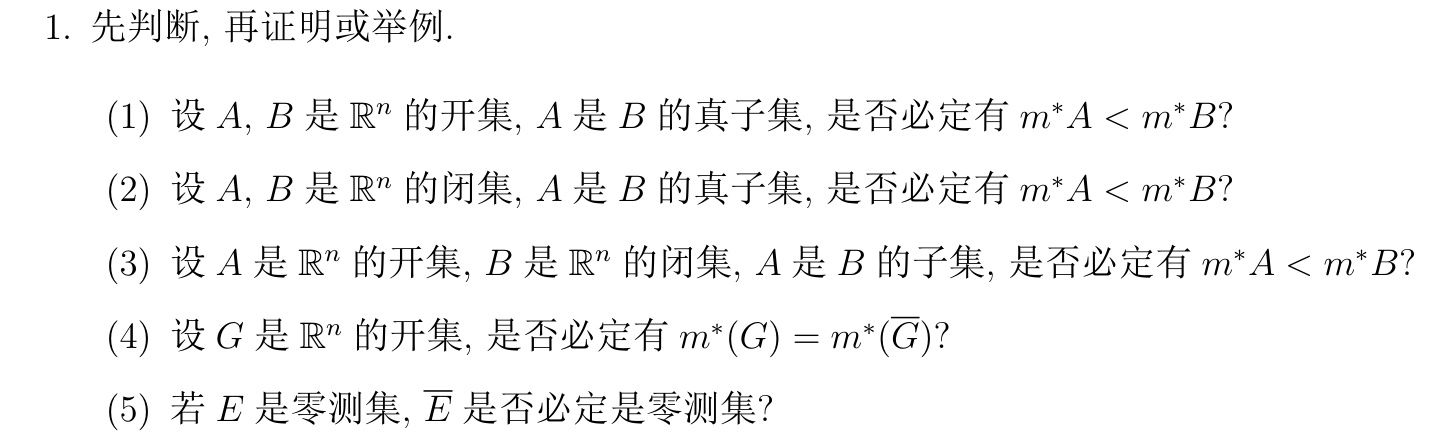
\includegraphics[width=\textwidth]{hw5-2025040310.png}
% \caption{}
\label{}
\end{figure}
(1) false. Let $A=(0,1)\cap \mathcal{C},B=(0,1)$, where $\mathcal{C}$ denotes the cantor set.

(2) false. Let $A=\varnothing,B=\mathcal{C}$.

(3) false. Let $A=\varnothing,B=\mathcal{C}$.

(4) true. By the definition of outer measure,
\[
m^{*}(G)\coloneqq \inf_{\{ I_k \}}\left\{  \sum_{k=1}^{\infty} l(I_k):\{ I_k \}\text{ covers }G  \right\}
\]
Then for any $\epsilon>0$, there exists a collection of nonempty open, bounded intervals $\{ I_k \}_{k=1}^{\infty}$ covering $G$, with
\[
\sum_{k=1}^{\infty} l(I_k)\leq m^{*}(G)+\epsilon
\]
In the general definition of outer measure defined on a sigma-algebra and by a set function, $I_k$ can be chosen to be closed. But here we construct a closed set from each $I_k$. Denote $I_k$ by $(a_k,b_k)$, let
\[
J_k\coloneqq (a_k-\epsilon/2^{k},b_k+\epsilon/2^{k})
\]
Then
\[
\overline{G}\subseteq  \overline{G\cap(a_k,b_k)}\subseteq[a_k,b_k]\subseteq (a_k-\epsilon/2^{k},b_k+\epsilon/2^{k})
\]
Thus $\{ J_k \}^{\infty}_{k=1}$ is a collection of open bounded nonempty intervals that covers $\overline{G}$. Therefore
\[
m^{*}(\overline{G})\leq \sum_{k=1}^{\infty}l(J_k)=\sum_{k=1}^{\infty} (l(I_k)+2\cdot\epsilon/2^{k}) =\sum_{k=1}^{\infty} l(I_k)+2\epsilon\leq m^{*}(G)+\epsilon
\]
Since $\epsilon$ is arbitrary, we have
\[
m^{*}(\overline{G})\leq m^{*}(G)
\]
Since $G\subseteq \overline{G}$, $m^{*}(G)\leq m^{*}(\overline{G})$,
\[
m^{*}(G)=m^{*}(\overline{G})
\]
(5) false. Let $E=\mathbb{Q}\cap(0,1)$, then $E$ is countable thus has measure zero, but $\overline{E}=(0,1)$ has measure $1$.

\begin{figure}[H]
\centering
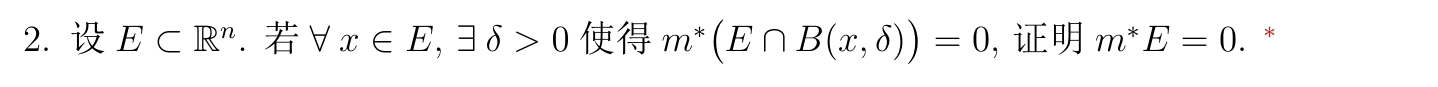
\includegraphics[width=\textwidth]{2-hw5-2025040310.png}
% \caption{}
\label{}
\end{figure}
Pick $r\in \mathbb{Q}\cap E$, then $\exists\delta_{r}>0$ such that $m^{*}(E\cap B(r,\delta_{r}))=0$. Therefore
\[
\begin{aligned}
m^{*}(E) & =m^{*}\left( E\cap\underbrace{ \left( \bigcup_{r\in \mathbb{Q}\cap E}B(r,\delta_{r}) \right) }_{ \text{covers }E } \right)=m^{*}\left( \bigcup_{r\in \underbrace{ \mathbb{Q}\cap E }_{ \text{countable} }}(E\cap B(r,\delta_{r})) \right) \\
 & \leq \sum_{r\in \mathbb{Q}\cap E}m^{*}(E\cap B(r,\delta_{r}))=\sum_{r\in \mathbb{Q}\cap E}0=0
\end{aligned}
\]
\begin{figure}[H]
\centering
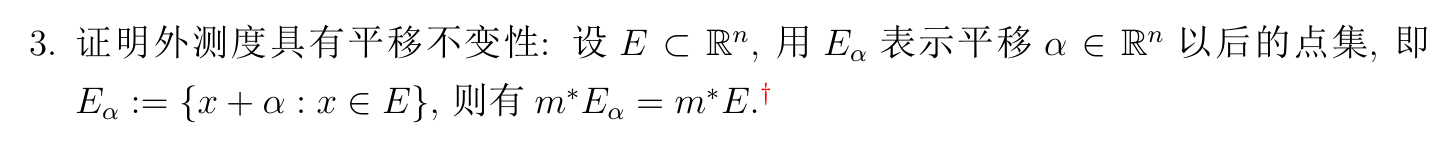
\includegraphics[width=\textwidth]{hw5-2025040311.png}
% \caption{}
\label{}
\end{figure}
\[
\begin{aligned}
m^{*}(E) & =\inf_{\{ I_k \}}\left\{  \sum_{k=1}^{\infty} l(I_k):\{ I_k \}\text{ covers }E  \right\} \\
 & =\inf_{\{ I_k+\alpha \} }\left\{  \sum_{k=1}^{\infty} l(I_k+\alpha): \{ I_k+\alpha \}\text{ covers }E_{\alpha}  \right\} \\
 & =m^{*}(E_{\alpha})
\end{aligned}
\]
\begin{figure}[H]
\centering
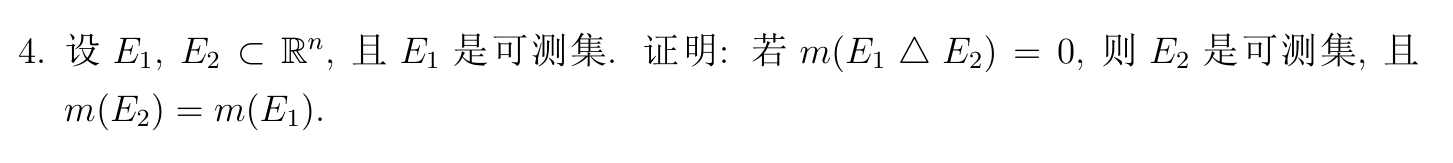
\includegraphics[width=\textwidth]{1-hw5-2025040311.png}
% \caption{}
\label{}
\end{figure}

Since
\[
E_2\subseteq E_1\cup(E_2\cap E_1^{c})\qquad E_2^{c}\subseteq E_1^{c}\cup(E_2^{c}\cap E_1)
\]
Then for any set $A$,
\[
\begin{aligned}
m^{*}(A\cap E_2) & \leq m^{*}(A\cap(E_1\cup(E_2\cap E_1^{c}))) \\
 & =m^{*}((A\cap E_1)\cup(\underbrace{ A\cap(E_2\cap E_1^{c})) }_{ \subseteq E_2\cap E_1^{c}\subseteq E_1\Delta E_2 }) \\
 & \leq m^{*}(A\cap E_1)+\underbrace{ m^{*}(E_1\Delta E_2) }_{ =m(E_1\Delta E_2) } \\
 & =m^{*}(A\cap E_1)
\end{aligned}
\]
\[
\begin{aligned}
m^{*}(A\cap E_2^{c}) & \leq m^{*}(A\cap(E_1^{c}\cup(E_2^{c}\cap E_1))) \\
 & =m^{*}((A\cap E_1^{c})\cup(A\cap(E_2^{c}\cap E_1))) \\
 & \leq m^{*}(A\cap E_1^{c})+m^{*}(E_1\Delta E_2) \\
 & = m^{*}(A\cap E_1^{c})
\end{aligned}
\]
Therefore
\[
m^{*}(A)\overset{ E_1\in \mathcal{M} }{ = }m^{*}(A\cap E_1)+m^{*}(A\cap E_1^{c})\geq m^{*}(A\cap E_2)+m^{*}(A\cap E_2^{c})
\]
Thus $E_2\in \mathcal{M}$.

\begin{figure}[H]
\centering
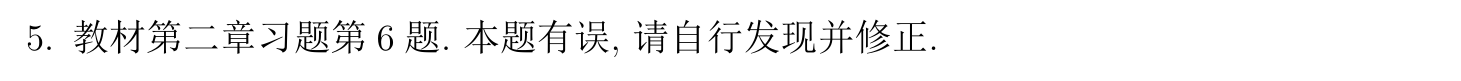
\includegraphics[width=\textwidth]{2-hw5-2025040311.png}
% \caption{}
\label{}
\end{figure}
\begin{figure}[H]
\centering
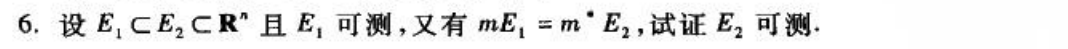
\includegraphics[width=\textwidth]{3-hw5-2025040311.png}
% \caption{}
\label{}
\end{figure}

Errata: $m^{*}E_2<\infty$.

For any set $A$,
\[
\begin{aligned}
m^{*}(A\cap E_2) & \leq  m^{*}(A\cap E_1)+m^{*}(A\cap E_2\cap E_1^{c}) \\
 & \leq m^{*}(A\cap E_1)+m^{*}(E_2\cap E_1^{c}) \\
 & \overset{ E_1\in \mathcal{M} }{ \leq  } m^{*}(A\cap E_1)+\underbrace{ m^{*}(E_2) }_{ =m(E_1) }-m^{*}(\underbrace{ E_2\cap E_1 }_{ =E_1 }) \\
 & =m^{*}(A\cap E_1)
\end{aligned}
\]
\[
m^{*}(A\cap E_2^{c})\leq m^{*}(A\cap E_1^{c})
\]
Therefore
\[
m^{*}(A)=m^{*}(A\cap E_1)+m^{*}(A\cap E_1^{c})\geq m^{*}(A\cap E_2)+m^{*}(A\cap E_2^{c})
\]
Hence $E_2\in \mathcal{M}$.

\begin{figure}[H]
\centering
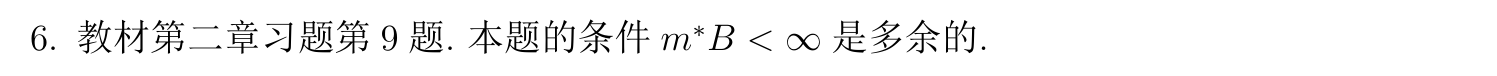
\includegraphics[width=\textwidth]{4-hw5-2025040311.png}
% \caption{}
\label{}
\end{figure}
\begin{figure}[H]
\centering
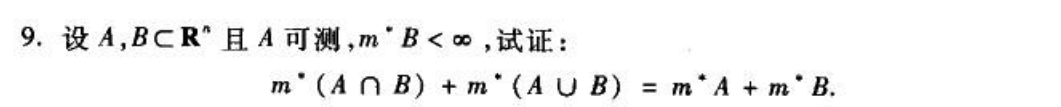
\includegraphics[width=\textwidth]{5-hw5-2025040311.png}
% \caption{}
\label{}
\end{figure}

If $m^{*}B=\infty$, then the equality is trivial. If $m^{*}B<\infty$, since $A\in \mathcal{M}$, then
\[
m^{*}B=m^{*}(A\cap B)+m^{*}(B\cap A^{c})
\]
\[
m^{*}(A\cup B)=m^{*}((A\cup B)\cap A)+m^{*}((A\cup B)\cap A^{c})=m^{*}A+m^{*}(B\cap A^{c})
\]
Hence
\[
m^{*}(A\cap B)+m^{*}(A\cup B)=m^{*}A+m^{*}B
\]
\begin{figure}[H]
\centering
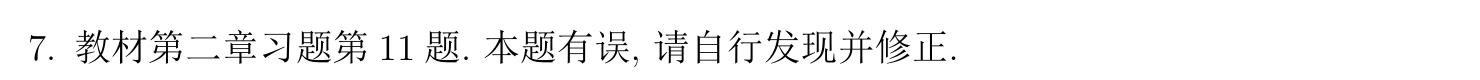
\includegraphics[width=\textwidth]{6-hw5-2025040311.png}
% \caption{}
\label{}
\end{figure}
\begin{figure}[H]
\centering
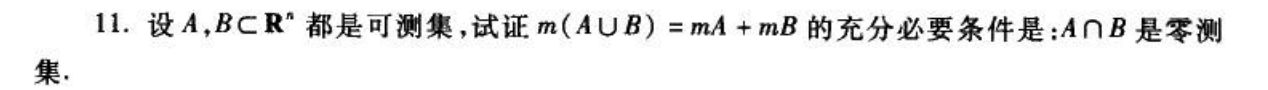
\includegraphics[width=\textwidth]{7-hw5-2025040311.png}
% \caption{}
\label{}
\end{figure}

Errata: $m^{*}A,m^{*}B<\infty$.

Since $A, B\in \mathcal{M}$, then
\[
m(A\cap B)+m(A\cup B)=mA+mB
\]
Then
\[
m(A\cup B)=mA+mB\iff m(A\cap B)=0
\]
\begin{figure}[H]
\centering
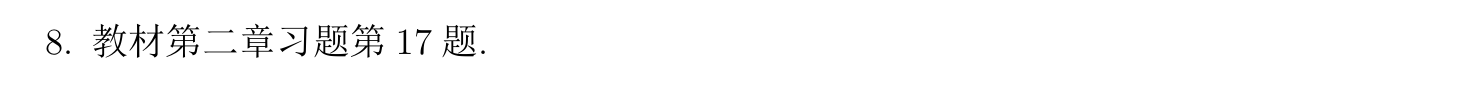
\includegraphics[width=\textwidth]{8-hw5-2025040311.png}
% \caption{}
\label{}
\end{figure}
\begin{figure}[H]
\centering
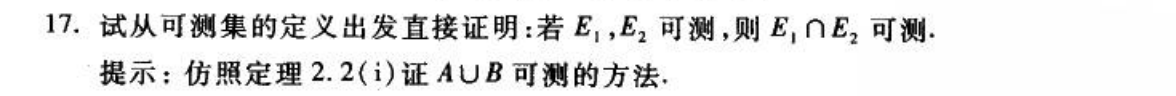
\includegraphics[width=\textwidth]{9-hw5-2025040311.png}
% \caption{}
\label{}
\end{figure}

For any set $A$,
\[
\begin{aligned}
 & m^{*}(A\cap E_1\cap E_2)+m^{*}(\underbrace{ A\cap(E_1\cap E_2)^{c} }_{ =(A\cap E_1^{c})\cup(A\cap E_2^{c}) })  \\
 = & m^{*}(A\cap E_1)-m^{*}(A\cap E_1\cap E_2)+m^{*}(A\cap E_1^{c})+m^{*}(A\cap E_2^{c})-m^{*}(A\cap E_1^{c}\cap E_2^{c}) \\
= & m^{*}A
\end{aligned}
\]
\begin{figure}[H]
\centering
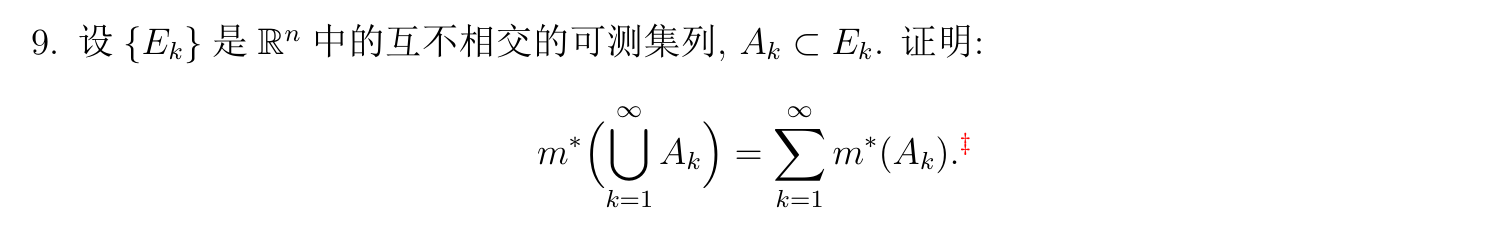
\includegraphics[width=\textwidth]{10-hw5-2025040311.png}
% \caption{}
\label{}
\end{figure}
\[
\begin{aligned}
m^{*}\left( \bigcup_{k=1}^{\infty} A_k \right) & =m^{*}\left( \left( \bigcup_{k=1}^{\infty} A_k \right)\cap E_1 \right)+m^{*}\left( \left( \bigcup_{k=1}^{\infty}  A_k \right)\cap E_1^{c} \right) \\
 & =m^{*}(A_1)+m^{*}\left( \bigcup_{k=2}^{\infty} A_k \right) \\
 & =m^{*}(A_1)+m^{*}(A_2)+m^{*}\left( \bigcup_{k=3}^{\infty}A_k  \right) \\
 & =\dots \\
 & =\sum_{k=1}^{\infty} m^{*}(A_{k})
\end{aligned}
\]
\begin{figure}[H]
\centering
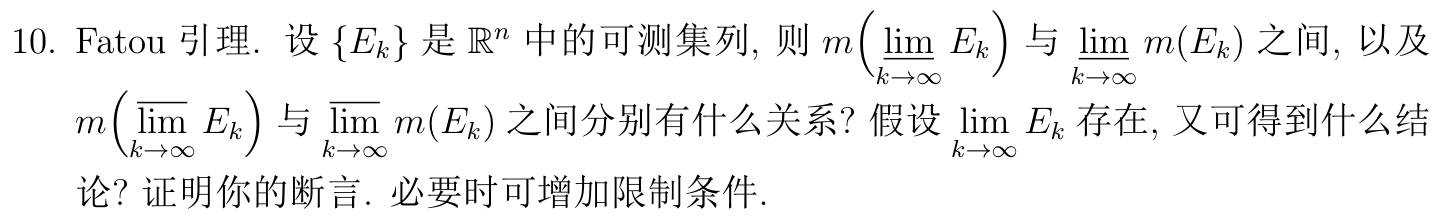
\includegraphics[width=\textwidth]{11-hw5-2025040311.png}
% \caption{}
\label{}
\end{figure}
\[
m(\varliminf_{ k \to \infty } E_k)=m\left( \bigcup_{k=1}^{\infty} \bigcap_{n=k}^{\infty} E_n \right)=\lim_{ k \to \infty } m\left(\underbrace{  \bigcap_{n=k}^{\infty} E_n }_{ \subseteq E_n,\forall n\geq k } \right)\leq \lim_{ k \to \infty } \inf_{n\geq k}m(E_n)=\varliminf_{ k \to \infty } m(E_k)
\]
\[
m(\varlimsup_{ k \to \infty } E_k)=m\left( \bigcap_{k=1}^{\infty} \bigcup_{n=k}^{\infty} E_n \right)=\lim_{ k \to \infty } m\left( \underbrace{ \bigcup_{n=k}^{\infty} E_n }_{ \supseteq E_n,\forall n\geq k } \right)\geq \lim_{ k \to \infty } \sup_{n\geq k}m(E_n)=\varlimsup_{ k \to \infty } m(E_k)
\]
When $\lim_{ k \to \infty }E_k$ exists, we have $m(\varlimsup_{ k \to \infty }E_k)=m(\varliminf_{ k \to \infty }E_k)$, then
\[
m(\varliminf_{ k \to \infty } E_k)\leq \varliminf_{ k \to \infty } m(E_k)\leq \varlimsup_{ k \to \infty } m(E_k)\leq m(\varlimsup_{ k \to \infty } E_k)=m(\varliminf_{ k \to \infty } E_k)
\]
Thus $\varlimsup_{ k \to \infty }m(E_k)=\varliminf_{ k \to \infty }m(E_k)$, and
\[
\lim_{ k \to \infty }m(E_k)=m(\lim_{ k \to \infty }E_k)
\]
\begin{figure}[H]
\centering
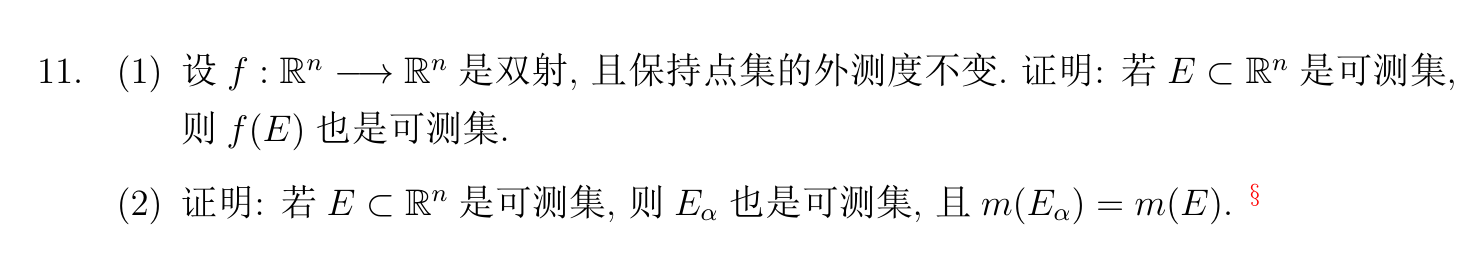
\includegraphics[width=\textwidth]{12-hw5-2025040311.png}
% \caption{}
\label{}
\end{figure}
(1)
Claim that:

\begin{enumerate}
	\item $f (B)\cap f (E)=f (B\cap E),\forall B, E\subset \mathbb{R}^{n}$.
	\item $f(E)^{c}=f(E^{c}),\forall E\subset \mathbb{R}^{n}$.
\end{enumerate}

Firstly, $f(B\cap E)\subseteq f(B)\cap f(E)$ is trivial. $\forall x\in f(B)\cap f(E)$, since $f$ is bijection, $\exists y\in B$ s.t. $x=f(y)$, $\exists z\in E$ s.t.$x=f(z)$. But the preimage of $x$ is unique, thus $y=z\in B\cap E$, thus $x\in f(B\cap E)$. Therefore $f(B)\cap f(E)=f(B\cap E)$.

Secondly, $\forall x\in f(E^{c})$, $x=f(y)$ for some $y\in E^{c}$, then $x\centernot{\in}f(E)$, then $x\in f(E)^{c}$, $f(E^{c})\subseteq f(E)^{c}$. $\forall x\in f(E)^{c}$, $x\neq f (y),\forall y\in E$. Since $f$ is bijection, $\exists z\in \mathbb{R}^{n}$ s.t.$x=f(z)$. Clearly $z\centernot{\in}E$, thus $z\in E^{c}$, $f(E)^{c}\subseteq f(E^{c})$. Therefore $f(E)^{c}=f(E^{c})$.

Then for any set $A\subset \mathbb{R}^{n}$, its preimage is $B$, i.e.$B=f^{-1}(A)$. Then
\[
\begin{aligned}
m^{*}(A\cap f(E))+m^{*}(A\cap (f(E)^{c})) & = m^{*}(f(B)\cap f(E))+m^{*}(f(B)\cap(f(E)^{c})) \\
 & =m^{*}(f(B\cap E))+m^{*}(f(B\cap E^{c})) \\
 & =m^{*}(B\cap E)+m^{*}(B\cap E^{c}) \\
 & \overset{ E\in \mathcal{M} }{ = }m^{*}B \\
 & =m^{*}(f(B)) \\
 & =m^{*}A
\end{aligned}
\]
Thus $f(E)$ is measurable.

(2) Since the outer measure $m^{*}$ is invariant under translation, the measure $m=\left.m^{*}\right|_{\mathcal{M}}$ is also invariant under translation.
